\section{Группа точек эллиптической кривой над полем}
\selectlanguage{russian}

\subsection{Группы точек на эллиптических кривых}

Эллиптическая кривая $E$ над полем вещественных чисел записывается в виде уравнения, связывающего координаты $x$ и $y$ точек кривой:

\begin{equation}
    E: ~ y^{2} = x^{3} + ax + b,
    \label{Wer}
\end{equation}

где $a,b \in \R$ -- вещественные числа. Эта форма представления эллиптической кривой называется формой Вейерштрасса.

На кривой определен инвариант

\begin{equation}
    J(E)=1728\frac{4a^{3} }{4a^{3} +27b^{2} }
    %\label{Inv}
\end{equation}

Пусть $x_{1} ,x_{2} ,x_{3} $ -- корни уравнения $x^3 + a x + b = 0$. Определим дискриминант $D$ в виде
    \[ D =(x_1 - x_2)^2 (x_1 - x_3)^2 (x_2 - x_3)^2 = - 16(4 a^3 + 27 b^2) \].

Рассмотрим различные значения дискриминанта $D$ и соответствующие им кривые, которые представлены на рисунках~\ref{fig:elliptic-curve-1},~\ref{fig:elliptic-curve-2},~\ref{fig:elliptic-curve-3}.

\begin{enumerate}
    \item При $D>0$ график эллиптической кривой состоит из двух частей (см. рис.~\ref{fig:elliptic-curve-1}). Прямая, проходящая через точки $P(x_1, y_1)$ и $Q(x_2, y_2)$, обязательно пересечёт вторую часть кривой в точке с координатами $(x_3, \widetilde{y}_3)$, отображением которой является точка $R(x_3, y_3)$, где $y_3 = - \widetilde{y}_3$. Любые точки на кривой при $D>0$ являются элементами группы по сложению.
        \begin{figure}[!ht]
        	\centering
        	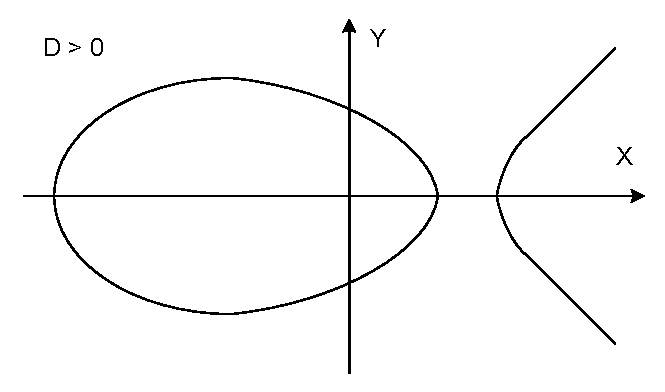
\includegraphics[width=0.5\textwidth]{pic/elliptic-curve-1}
            \caption{Эллиптическая кривая с дискриминантом $D>0$\label{fig:elliptic-curve-1}}
        \end{figure}
    \item Если $D=0$, то левая и правая части касаются в одной точке (см. рис.~\ref{fig:elliptic-curve-2}). Эти кривые называются сингулярными и не рассматриваются.
        \begin{figure}[!ht]
        	\centering
        	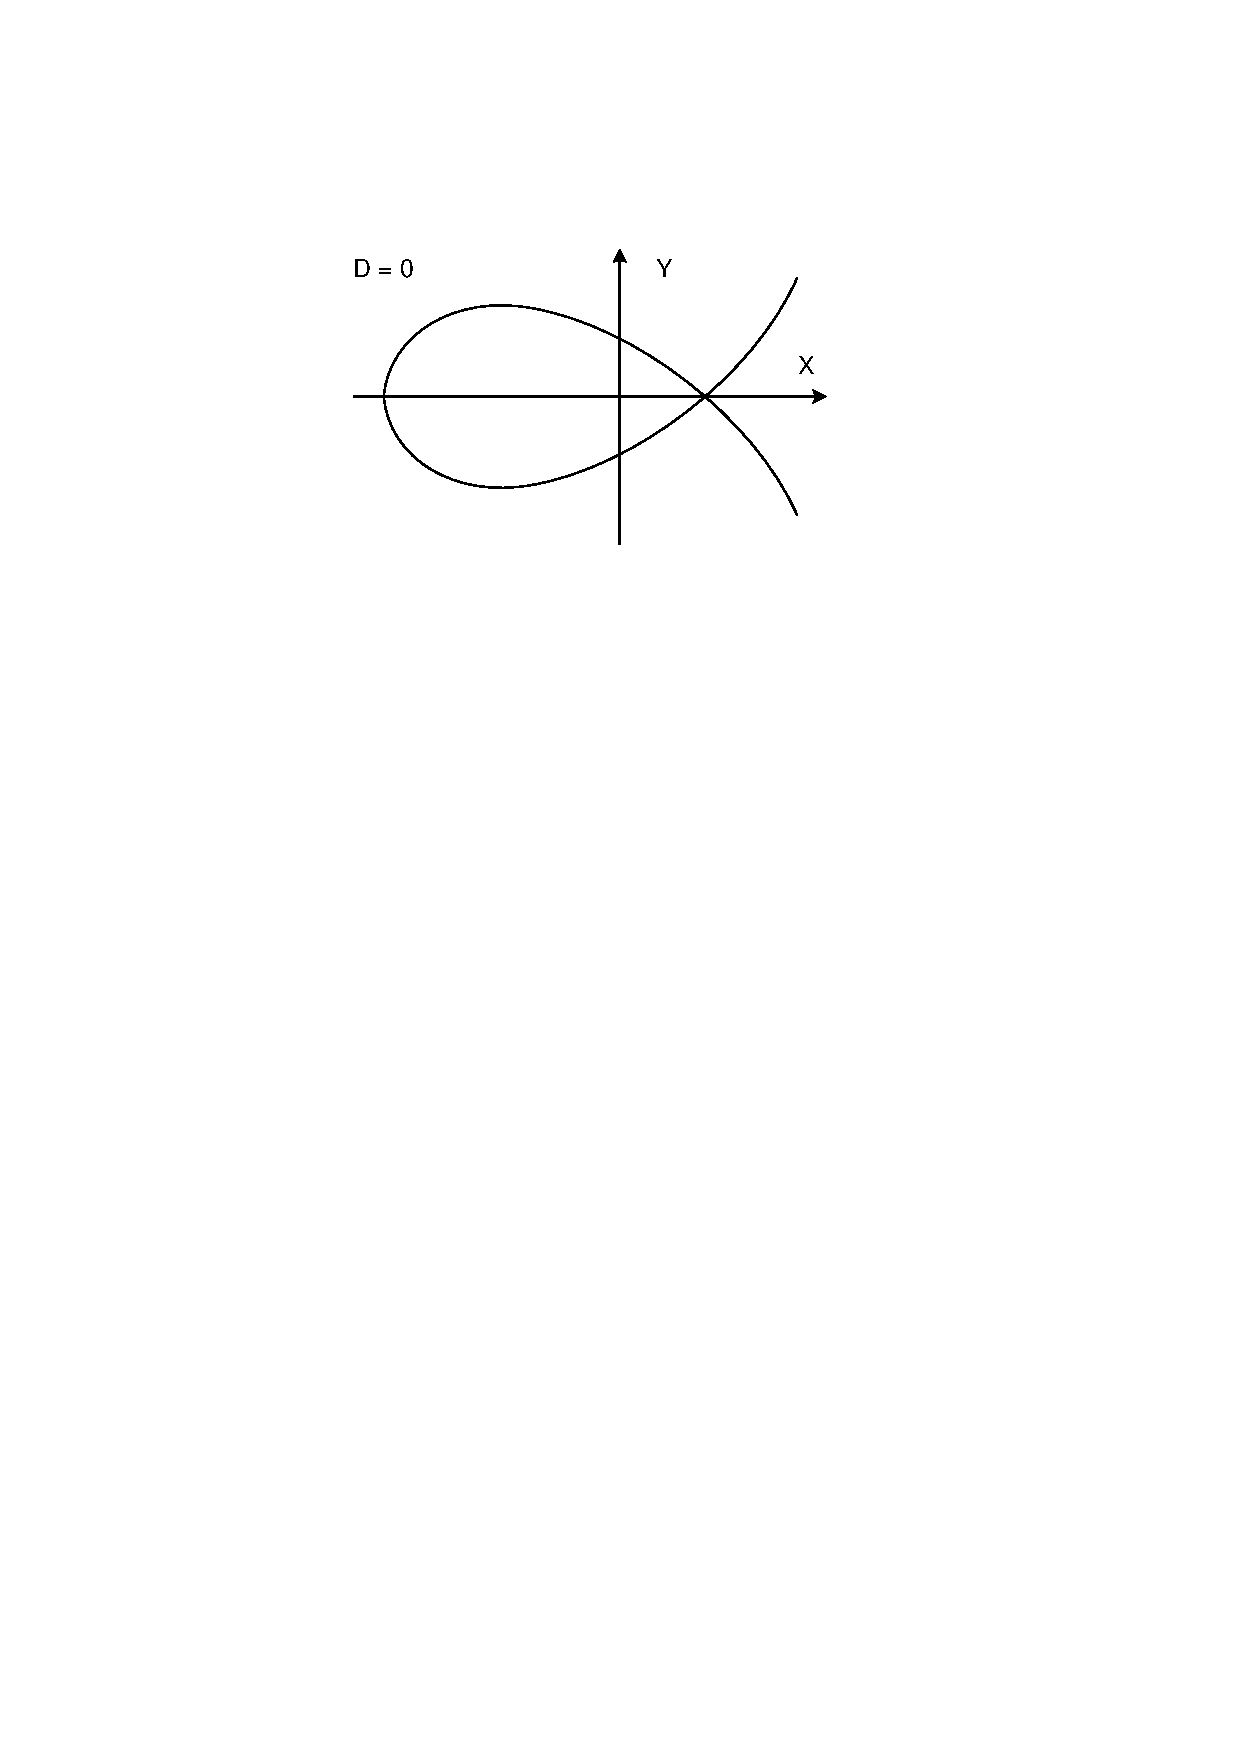
\includegraphics[width=0.5\textwidth]{pic/elliptic-curve-2}
            \caption{Эллиптическая кривая с дискриминантом $D = 0$\label{fig:elliptic-curve-2}}
        \end{figure}
    \item Если $D<0$, то записанное выше уравнение~\ref{Wer} описывает одну кривую, представленную на рис.~\ref{fig:elliptic-curve-3}.
        \begin{figure}[!ht]
        	\centering
        	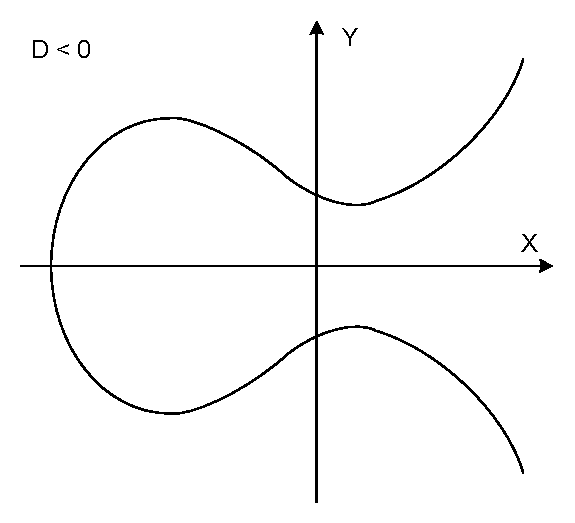
\includegraphics[width=0.5\textwidth]{pic/elliptic-curve-3}
            \caption{Эллиптическая кривая с дискриминантом $D < 0$\label{fig:elliptic-curve-3}}
        \end{figure}
\end{enumerate}

Рассмотрим операцию сложения точек на эллиптической кривой при $D>0$ (другие кривые не рассматриваются).

Пусть точки $P(x_1, y_1)$ и $Q(x_2, y_2)$ принадлежат эллиптической кривой (рис.~\ref{fig:elliptic-curve-1}). Определим операцию сложения точек
    \[ P + Q = R. \]

\begin{enumerate}
    \item Eсли $P \neq Q$, то точка $R$ определяется как отображение (инвертированная $y$-координата) точки, полученной пересечением эллиптической кривой и прямой $PQ$. Совместно решая уравнения кривой и прямой, можно найти координаты точки пересечения. Точка $R = (x_3, y_3)$ равна:
        \[ x_3 = \lambda^2 - x_1 - x_2, \]
        \[ y_3 = - y_1 + \lambda (x_1 - x_3), \]
        где
        \[ \lambda = \frac{y_2 - y_1}{x_2 - x_1} \]
        есть тангенс угла наклона между прямой, проходящей через точки $P$ и $Q$, и осью $x$.

        Теперь рассмотрим специальные случаи.
    \item Пусть точки совпадают: $P = Q$. Прямая $PQ$ превращается в касательную к кривой в точке $P$. Находим пересечение касательной с кривой, инвертируем $y$-координату полученной точки, это будет точка $P + P = R$. Тогда $\lambda$ -- тангенс угла между касательной, проведенной к эллиптической кривой в точке $P$, и осью $x$. Запишем уравнение касательной к эллиптической кривой в точке $(x,y)$ в виде
            \[ 2 y y' = 3 x^2 + a. \]
        Производная равна
            \[ y' = \frac{3 x^2 + a}{2 y} \]
        и
            \[ \lambda = \frac{3 x_1^2 + a}{2 y_1}. \]
        Координаты $R$ имеют прежний вид:
            \[ x_3 = \lambda^2 - x_1 - x_2, \]
            \[ y_3 = - y_1 + \lambda (x_1 - x_3), \]
    \item Пусть $P$ и $Q$ -- противоположные точки, то есть $P=(x,y)$ и $Q=(x, -y)$. Введём еще одну точку на бесконечности и обозначим ее $O$ (точка $O$ или точка 0 <<ноль>>, или альтернативное обозначение $\infty$). Результатом сложения двух противоположных точек определим точку $O$. Точка $Q$ в данном случае обозначается как $-P$:
        \[ P = (x,y), ~ -P = (x, -y), ~ P + (-P) = O. \]
    \item Пусть $P = (x, 0)$ лежит на оси $x$, тогда
        \[ -P = P, ~ P + P = O. \]
\end{enumerate}

Все точки эллиптической кривой, а также точка $O$, образуют коммутативную группу $\E(\R)$ относительно введенной операции сложения, то есть выполняются законы коммутативной группы\index{группа!точек эллиптической кривой}:
\begin{itemize}
    \item сумма точек $P + Q$ лежит на эллиптической кривой;
    \item существует нулевой элемент -- это точка $O$ на бесконечности:
        \[ \forall P \in \E(\R): ~ O + P = P; \]
    \item для любой точки $P$ существует единственный обратный элемент $-P$:
        \[ P + (-P) = O; \]
    \item выполняется ассоциативный закон:
        \[ (P + Q) + F = P + (Q + F) = P + Q + F; \]
    \item выполняется коммутативный закон:
        \[ P + Q = Q + P. \]
\end{itemize}

Сложение точки с самой собой $d$ раз обозначим как умножение точки на число $d$:
    \[ \underbrace{P + P + \ldots + P}_{d \text{ раз}} = d P. \]


\subsection{Эллиптические кривые над конечным полем}

Эллиптические кривые можно строить не только над полем рациональных чисел, но и над другими полями. То есть координатами точек могут выступать не только числа, принадлежащие полю рациональных чисел $\R$, но и элементы поля комплексных чисел $\mathbb{C}$ или конечного поля $\F$. В криптографии нашли своё применение эллиптические кривые именно над конечными полями.

Далее будем рассматривать эллиптические кривые над конечным полем, являющимся кольцом вычетов по модулю нечётного простого\index{число!простое} числа $p$ (дискриминант не равен 0):
    \[ E: ~ y^2 = x^3 + a x + b, \]
    \[ a, b, x, y \in \Z_p, \]
    \[ \Z_p = \{0, 1, 2,  \ldots,  p-1\}.\]

Возможна также более компактная запись:

    \[ E: ~ y^2 = x^3 + a x + b \mod p\]

Точкой эллиптической кривой является пара чисел
    \[ (x,y): x, y \in \Z_p, \]
удовлетворяющая уравнению эллиптической кривой, определённой над конечным полем $\Z_p$.

Операцию сложения двух точек $P = (x_1, y_1)$ и $Q = (x_2, y_2)$ определим точно так же, как и в случае кривой над полем вещественных чисел, описанным выше.

\begin{enumerate}
    \item Две точки $P = (x_1, y_1)$ и $Q = (x_2, y_2)$ эллиптической кривой, определённой над конечным полем $\Z_p$, складываются по правилу:
        \[
            P + Q = R \equiv (x_3, y_3),
        \] \[
            \left\{ \begin{array}{l}
                x_3 = \lambda^2 - x_1 - x_2 \mod p,\\
                y_3 = - y_1 + \lambda (x_1 - x_3) \mod p,\\
            \end{array} \right.
        \]
        где
        \[
            \lambda = \left\{ \begin{array}{l}
                \frac{y_2 - y_1}{x_2 - x_1} \mod p, ~ \text{ если } P \ne Q, \\
                \\
                \frac{3 x_1^2 + a}{2 y_1} \mod p, ~ \text{ если } P = Q. \\
            \end{array} \right.
        \]
    \item Сложение точки $P=(x,y)$ c противоположной точкой \\
        $(-P) = (x,-y)$ даёт точку в бесконечности $O$:
        \[ P + (-P) = O, \]
        \[ (x_1, y_1) + (x_1, -y_1) = O, \]
        \[ (x_1, 0) + (x_1, 0) = O. \]
\end{enumerate}

Мы рассматриваем эллиптические кривые над конечным полем $\Z_p$, где $p > 3$ -- простое\index{число!простое} число, элементы $\Z_p$ -- целые числа $\{0, 1, 2,  \ldots, p-1\}$, т.~е. исследуем следующее уравнение двух переменных $x, y \in \Z_p$:
    \[ y^2 = x^3 + a x + b \mod p, \]
где $a, b \in \Z_p$ -- некоторые константы.

Как и в случае выше, множество точек над конечным полем $\Z_p$, удовлетворяющих уравнению эллиптической кривой, вместе с точкой в бесконечности $O$ образуют конечную группу $\E(\Z_p)$ относительно описанного закона сложения:\index{группа!точек эллиптической кривой}
    \[ \E(\Z_p) ~ \equiv~  O ~ \bigcup ~
        \left\{ (x, y) \in \Z_p \times \Z_p ~\Big|~ y^2 = x^3 + a x + b \mod p \right\}. \]

По теореме Хассе\index{теорема!Хассе} порядок группы точек $|\E(\Z_p)|$ оценивается как
    \[ (\sqrt{p}-1)^2 \leq |\E(\Z_p)| \leq (\sqrt{p}+1)^2, \]
или в другой записи
    \[ \Big| |\E(\Z_p)| - p - 1 \Big| \le 2 \sqrt{p}. \]

\subsection{Примеры группы точек}

\subsubsection{Пример 1}

Пусть эллиптическая кривая задана уравнением
    \[ E: ~ y^2 = x^3 + 1 \mod 7. \]
Найдём все решения этого уравнения, а также количество точек $|\E(\Z_p)|$ на этой эллиптической кривой. Для нахождения решений уравнения составим следующую таблицу:

\begin{center} \begin{tabular}{|c|c|c|c|c|c|c|c|}
    \hline
    $x$ & 0 & 1 & 2 & 3 & 4 & 5 & 6 \\
    \hline
    $y^2$ & 1 & 2 & 2 & 0 & 2 & 0 & 0 \\
    \hline
    $y_1$ & 1 & 3 & 3 & 0 & 3 & 0 & 0 \\
    \hline
    $y_2 = - y_1 \mod p$ & 6 & 4 & 4 &   & 4 &   &   \\
    \hline
\end{tabular} \end{center}

Выпишем все точки, принадлежащие данной эллиптической кривой $\E(\Z_p)$:
\[
    \begin{array}{cccc}
        P_1 = O, & P_2 = (0,1), & P_3 = (0,6), & P_4 = (1,3), \\
        P_5 = (1,4), & P_6 = (2,3), & P_7 = (2,4), & P_8 = (3,0), \\
        P_9 = (4,3), & P_{10} = (4,4), & P_{11} = (5,0), & P_{12} = (6,0). \\
    \end{array}
\]

Получили
    \[ |\E(\Z_p)| = 12. \]

Проверим выполнение неравенства Хассе:
    \[ \left| 12 - 7 - 1 \right| = 4 < 2 \sqrt{7}. \]
Следовательно, неравенство Хассе выполняется.

Минимальное натуральное число $s$ такое, что
\[ \underbrace{P + P + \ldots + P}_{s} \equiv s P = O \]
будем называть \emph{порядком точки $P$}.

%Теорема Лагранжа определяет порядок подгруппы.

\subsubsection{Пример 2}

Группа точек эллиптической кривой
    \[ y^2 = x^3 + 5 x + 6 \mod 17 \]
состоит из точек
\[ \begin{array}{ccccccc}
    \E(\Z_p) & =~ \Big\{ & (-8, \pm 7), & (-7, \pm 6), & (-6, \pm 7), &   & \\
             &           & (-5, \pm 3), & (-3, \pm 7), & (-1, 0),     & O & \Big\}. \\
\end{array} \]

Порядок группы:
    \[ |\E(\Z_p)| = 12. \]

Порядок группы точек по теореме Хассе:
    \[ (\sqrt{p}-1)^2 \leq |\E(\Z_p)| \leq (\sqrt{p}+1)^2, \]
    \[ 10 \leq 12 \leq 26. \]

Порядки возможных подгрупп: 2, 3, 4, 6 (все возможные делители порядка группы 12).

В табл.~\ref{tab:ellipic-point-order-sample} найден порядок точки $P = (-8, 7)$ той же кривой
    \[ y^2 = x^3 + 5 x + 6 \mod 17. \]
Проверяются только степени точки, равные всем делителям порядка группы 12, отличным от 1: 2, 3, 4, 6. Найденный порядок точки $(-8,7)$ равен 12, следовательно, она -- генератор всей группы.

\begin{table}[!ht]
    \centering
    \caption{Пример нахождения порядка точки\label{tab:ellipic-point-order-sample}}
    \resizebox{\textwidth}{!}{ \begin{tabular}{|c|p{0.9\textwidth}|}
        \hline
        2 & $2 P = P + P = 2 \cdot (-8,7) = (-8,7) + (-8,7) = R$, \\
        & $\lambda = \frac{3 x_P^2 + a}{2y_P} = \frac{3 \cdot (-8)^2 + 5}{2 \cdot 7} = 8 \mod 17$, \\
        & $x_R = \lambda^2 - 2x_P = 8^2 - 2 \cdot (-8) = -5 \mod 17$, \\
        & $y_R = \lambda (x_P - x_R) - y_P = 8 \cdot ((-8) - (-5)) - 7 = 3 \mod 17$, \\
        & $R = 2P = (-5, 3)$ \\
        \hline
        3 & $3 P = 2 P + P = Q + P = R$, \\
        & $Q = 2P = (-5, 3)$, \\
        & $\lambda = \frac{y_Q - y_P}{x_Q - x_P} = \frac{3 - 7}{-5 - (-8)} = -7 \mod 17$, \\
        & $x_R = \lambda^2 - x_P - x_Q = (-7)^2 - (-8) - (-5) = -6 \mod 17$, \\
        & $y_R = \lambda (x_P - x_R) - y_P = -7 \cdot (-8 - (-6)) - 7 = 7 \mod 17$, \\
        & $R = 3P = (-6, 7)$ \\
        \hline
        4 & $4 P = 2 \cdot (2 P) = 2 \cdot (-5,3) = (-3, -7)$ \\
        \hline
        6 & $6 P = 2 P +  4 P = (-5,3) + (-3, -7) = (-1, 0)$ \\
        \hline
        12 & $12 P = 2 \cdot (6 P) = 2 \cdot (-1, 0) = O$ \\
        \hline
    \end{tabular} }
\end{table}

В табл.~\ref{tab:elliptic-group-sample} найдены порядки точек и циклические подгруппы группы точек $\E(\Z_p)$ такой же эллиптической кривой
    \[ y^2 = x^3 + 5 x + 6 \mod 17. \]
Группа циклическая, число генераторов:
    \[ \varphi(12) = 4. \]
Циклические подгруппы:
    \[ \Gr^{(2)}, ~ \Gr^{(3)}, ~ \Gr^{(4)}, ~ \Gr^{(6)}, \]
верхний индекс обозначает порядок подгруппы.

\begin{table}[!ht]
    \centering
    \caption{Генераторы и циклические подгруппы группы точек эллиптической кривой\label{tab:elliptic-group-sample}}
    \resizebox{\textwidth}{!}{
    \begin{tabular}{|c|l|c|}
        \hline
        Элемент & Порождаемая группа или подгруппа & Порядок \\
        \hline
        $(-8,  \pm 7) $ & Вся группа $\E(\Z_p)$ & 12, генератор \\
        $(-7, \pm 6) $ & Вся группа $\E(\Z_p)$ & 12, генератор \\
        $(-6, \pm 7) $ & $\Gr^{(4)} ~=~ \big\{ ~ (-6, \pm 7), ~ (-1,0), ~ O ~ \big\}$ & 4 \\
        $(-5, \pm 3) $ & $\Gr^{(6)} ~=~ \big\{ ~ (-5, \pm 3), ~ (-3, \pm 7), ~ (-1,0), ~ O ~ \big\}$ & 6 \\
        $(-3, \pm 7) $ & $\Gr^{(3)} ~=~ \big\{ ~ (-3, \pm 7), ~ O ~ \big\}$ & 3\\
        $(-1, 0)     $ & $\Gr^{(2)} ~=~ \big\{ ~ (-1, 0), ~ O ~ \big\}$ & 2\\
        \hline
    \end{tabular}
    }
\end{table}
